\documentclass{article}
%
\usepackage{mathbbol}

\usepackage{ctex}
\usepackage{geometry}
\usepackage[dvipsnames, svgnames, x11names]{xcolor}
\usepackage[mathscr]{euscript}
\usepackage{tikz}
\usepackage{xstring}
%

\usetikzlibrary{decorations.pathreplacing}
\usetikzlibrary{positioning, arrows.meta, automata}
%
%
\begin{document}
%
\begin{center}
  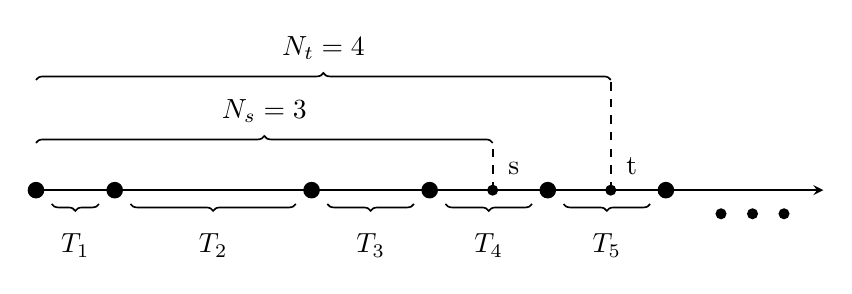
\begin{tikzpicture}[->,>=stealth,node distance=2cm,semithick,initial text=,]
    
  \draw[->] (-5,0) to (5,0);
  \fill (-5,0) circle (3pt);
  \fill (-4,0) circle (3pt);
  \fill (-1.5,0) circle (3pt);
  \fill (-0,0) circle (3pt);
  \fill (1.5,0) circle (3pt);
  \fill (3,0) circle (3pt);
  \fill (4.5,-0.3) circle (2pt);
  \fill (4.1,-0.3) circle (2pt);
  \fill (3.7,-0.3) circle (2pt);
  \fill (0.8,0) circle (2pt) node [above right = 0.1cm]{s};
  \fill (2.3,0) circle (2pt) node [above right = 0.1cm]{t};

  \draw[-,decorate, decoration={brace,mirror,raise=5pt}] (-4.8,0)--(-4.2,0) node[midway, yshift=-20pt]{$T_1$};
  \draw[-,decorate, decoration={brace,mirror,raise=5pt}] (-3.8,0)--(-1.7,0) node[midway, yshift=-20pt]{$T_2$};
  \draw[-,decorate, decoration={brace,mirror,raise=5pt}] (-1.3,0)--(-0.2,0) node[midway, yshift=-20pt]{$T_3$};
  \draw[-,decorate, decoration={brace,mirror,raise=5pt}] (0.2,0)--(1.3,0) node[midway, yshift=-20pt]{$T_4$};
  \draw[-,decorate, decoration={brace,mirror,raise=5pt}] (1.7,0)--(2.8,0) node[midway, yshift=-20pt]{$T_5$};

  \draw[-,decorate, decoration={brace, raise=0.6cm}] (-5.0,0)--(0.8,0) node[midway, yshift=1.0cm]{$N_s=3$};
  \draw[-,decorate, decoration={brace, raise=1.4cm}] (-5.0,0)--(2.3,0) node[midway, yshift=1.8cm]{$N_t=4$};

  \draw[-, dashed] (0.8,0) to (0.8,0.6);
  \draw[-, dashed] (2.3,0) to (2.3,1.4);

  
  

  \end{tikzpicture}
  \heiti\\ 图8.18 事件序列\songti
\end{center}
%
\end{document}
